%%%%%%%%%%%%%%%%%%%%%%%%%%%%%%%%%%%%%%%%%
% Structured General Purpose Assignment
% LaTeX Template
%
% This template has been downloaded from:
% http://www.latextemplates.com
%
% Original author:
% Ted Pavlic (http://www.tedpavlic.com)
%
% Note:
% The \lipsum[#] commands throughout this template generate dummy text
% to fill the template out. These commands should all be removed when 
% writing assignment content.
%
%%%%%%%%%%%%%%%%%%%%%%%%%%%%%%%%%%%%%%%%%

\documentclass{article}

\usepackage{fancyhdr} % Required for custom headers
\usepackage{lastpage} % Required to determine the last page for the footer
\usepackage{extramarks} % Required for headers and footers
\usepackage{graphicx} % Required to insert images
\usepackage[utf8]{inputenc}

% Margins
\topmargin=-0.45in
\evensidemargin=0in
\oddsidemargin=0in
\textwidth=6.5in
\textheight=9.0in
\headsep=0.25in 

\linespread{1.1} % Line spacing



\setlength\parindent{0pt} % Removes all indentation from paragraphs

%----------------------------------------------------------------------------------------
%	DOCUMENT STRUCTURE COMMANDS
%	Skip this unless you know what you're doing
%----------------------------------------------------------------------------------------

% Header and footer for when a page split occurs within a problem environment
\newcommand{\enterProblemHeader}[1]{
\nobreak\extramarks{#1}{#1 continued on next page\ldots}\nobreak
\nobreak\extramarks{#1 (continued)}{#1 continued on next page\ldots}\nobreak
}

% Header and footer for when a page split occurs between problem environments
\newcommand{\exitProblemHeader}[1]{
\nobreak\extramarks{#1 (continued)}{#1 continued on next page\ldots}\nobreak
\nobreak\extramarks{#1}{}\nobreak
}

\setcounter{secnumdepth}{0} % Removes default section numbers
\newcounter{homeworkProblemCounter} % Creates a counter to keep track of the number of problems

%----------------------------------------------------------------------------------------
%	NAME AND CLASS SECTION
%----------------------------------------------------------------------------------------

\newcommand{\lessonNumber}[1]{Lezione\ \##1} % Assignment title
\newcommand{\lessonDate}[4]{#1,\ #2\ #3\ #4} % Due date
\newcommand{\lessonCourse}[1]{#1} % Course/class
\newcommand{\lessonTime}[1]{#1} % Class/lecture time
\newcommand{\lessonTeacher}[1]{#1} % Teacher/lecturer
\newcommand{\lessonAuthor}[1]{#1} % Your name
\begin{document}

\section{Documentazione (10)}

La documentazione deve essere una conseguenza dei processi organizzativi. Serve documentare nel modo meno intrusivo possibile. Fra le cose più importanti che fa la documentazione è fornire una misura sull'avanzamento del progetto (Piano di progetto), che fornisce dei \textbf{consuntivi} (stato fotografato) e \textbf{preventivi} (stime). I consuntivi sono finali se siamo alla fine del progetto, o parziali se siamo in corso.\\
Documentare serve per dominare la complessità dei processi produttivi, attenuare la volatilità dei requisiti, facilitare il controllo di avanzamento.\\

Misureremo le cose sulle quali possiamo e vogliamo fissare degli obiettivi di miglioramento. Misurazione per obiettivi, "ad hoc". Il responsabile di progetto deve avere un ``\textit{cruscotto}'' con gli indicatori delle metriche che utilizziamo, e questi indicatori devono essere aggiornati. Vogliamo inoltre che il responsabile spenda il meno possibile, per far questo devo documentare tutte le attività di pianificazione, gestione, sviluppo, verifica e validazione. Il piano ci dà degli obiettivi sui tempi e costi, le norme sono invece gli strumenti e le procedure che uso per rendere il piano fattibile. Il primo e più importante documento da realizzare (interno) sono le \textbf{norme di progetto}, che cresceranno nel tempo. Un altro documento importante è la specifica software, che è la descrizione ad alto livello del sistema.\\
Ogni architettura sw ha molte viste:

\begin{itemize}

	\item \textbf{Modello statico:} Identifica le componenti principali e procede per decomposizione grafica;
	\item \textbf{Modello dinamico:} Illustra la struttura a processi del sistema;
	\item \textbf{Modello delle interfacce:} Definisce le interfacce  del sistema;
	\item \textbf{Modello delle relazioni:} Identifica il flusso dei dati tra componenti distinti in relazione tra loro;
	\item \textbf{Modello di distribuzione:} Associazione tra nodi fisici e componenti logiche.

\end{itemize}

L'architettura va descritta in due documenti distinti:

\begin{itemize}

	\item \textbf{Specifica tecnica} fissa linee e strategie di realizzazione, avvia la fase realizzativa ma non fissa i dettagli implementativi. Per ogni componente specifica la funzione svolta (con quali strutture dati, quali e quanti flussi di controllo) il tipo di dati in ingresso, in uscita, risorse logiche e fisiche necessarie per il suo funzionamento;
	\item \textbf{Definizione di prodotto:} consente di stimare costo e tempi di realizzazione,  consente sviluppo parallelo dei componenti terminali. Decompone i componenti architetturali in moduli a grana fine finché ogni modulo ha dimensione, coesione, complessità e accoppiamento appropriati per la codifica in parallelo. In oltre questo documento deve fornire tutti i dettagli necessari alla codifica e alla verifica di ciascun modulo.

\end{itemize}

\begin{center}
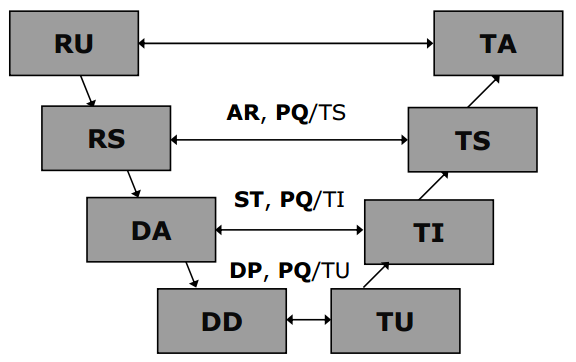
\includegraphics[width=0.4\columnwidth]{img1}
\end{center}
\texttt{Tutto ciò che facciamo in discesa implica ciò che faremo in salita, e tutto ciò che facciamo in salita motiva quello che sta in discesa.} \\
Per la documentazione si procede in modo \textbf{sequenziale}. In questo modo si suddividono i moduli grandi, in modo da agevolare i programmatori, i quali produrranno tanti moduli e li integreranno tra loro dopo la validazione. Dentro il repository si devono caricare moduli già verificati in modo automatico e/o manuale (preferibilmente automatico perché la verifica manuale costa).\\
La progettazione di dettaglio fissa unità, fissa ciò che troveremo nel \textit{ramo ascendente}. Quando ho unità buone le posso integrare (test di integrazione). Quando tutte le parti sono messe insieme allora posso fare un test di sistema. Nel percorso discendente il lavoro che riguarda la qualità deve includere specifiche progressive delle verifiche che farò per la produzione.\\

Stadi di preparazione dei documenti:

\begin{itemize}

	\item \textbf{Creazione}
	\item \textbf{Pulitura}
	\item \textbf{Rilascio}

\end{itemize}

Il \textbf{tracciamento dei requisiti}  fissa la relazione tra i prodotti del processo di sviluppo, tramite matrici di tracciabilità. Può essere fatto:

\begin{itemize}

	\item \textbf{Foward:} in avanti (completezza), "non mi dimentico niente", ciascun ingresso a una fase deve essere messo in relazione con una specifica uscita di quella fase, fatto attraverso \textbf{matrici di tracciabilità};
	\item \textbf{Backward:} all'indietro (necessità), ciascuna uscita di una fase deve essere messa in relazione con uno specifico ingresso a quella fase.
\end{itemize}




Il tracciamento deve essere assicurato ed automatizzato il più possibile. Dobbiamo avere \textbf{evidenza di copertura}. E' un lavoro potenzialmente oneroso e non può essere fatto a mano. I requisiti andranno identificati attraverso codici che li renderanno \textbf{univoci}. Un codice che definisca di cosa stiamo parlando (es. RU). Poi dovrò numerarli in modo gerarchico, in cui c'è uno spazio e un ambito. Non un numero in modo sequenziale ma raggruppato attorno a \textbf{categorie}. Non devo avere necessariamente solo numeri ma posso avere anche lettere.\\

\textbf{Manuale utente:} deve essere adatto alle caratteristiche dell'utente e alle caratteristiche dell'interfaccia utente. Un manuale serve come informazione supplementare. Si usa uno stile molto succinto e sintetico, non narrativo. \\

\end{document}